\section{Method}
\label{sec:methodology}

\subsection{Architecture}
\label{sec:arch_overview}
The detector predicts boxes for four classes: \texttt{worker}, \texttt{forklift}, \texttt{pallet\_truck}, and \texttt{amr}. It keeps the YOLO11s backbone (Layers 0--9, ending with \texttt{SPPF}), its FPN/PAN neck, and its decoupled anchor-free \texttt{Detect} head, trained with the Ultralytics CIoU, binary cross-entropy, and distribution focal losses. In \textbf{SS2D-P5}, the \texttt{C2PSA} block at Layer~10 is replaced by a shape-compatible \texttt{WarehouseSS2DBlock}, $[b, 512, 20, 20] \to [b, 512, 20, 20]$, at stage $P_5$. \textbf{SS2D-P4P5} adds a second block at $P_4$ ($[b, 256, 40, 40]$, Layer~7). Fig.~\ref{fig:arch_diagram} shows the block.

\begin{figure}[t]
\centering
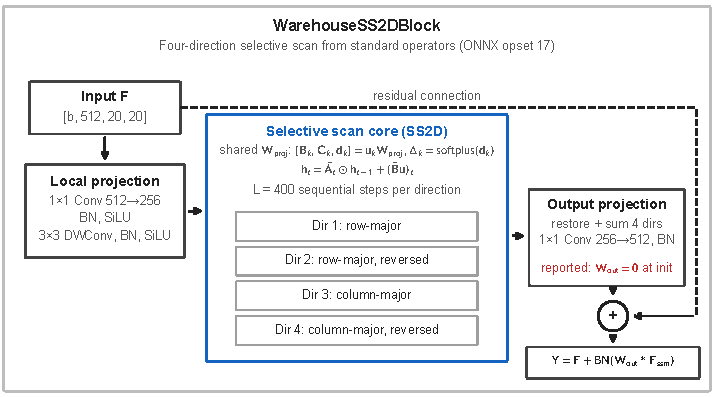
\includegraphics[width=\textwidth]{figures/fig_ss2d_block.pdf}
\caption{The \texttt{WarehouseSS2DBlock} that replaces \texttt{C2PSA} at Layer~10. The red label marks the $\mathbf{W}_{\text{out}} = \mathbf{0}$ initialization used for all reported models (Eq.~\eqref{eq:zero_wout}).}
\label{fig:arch_diagram}
\end{figure}

\subsection{Warehouse SS2D Block}
\label{sec:mamba_integration}
A $1 \times 1$ convolution projects the $C_{\text{in}} = 512$ input channels of $\mathbf{F}$ to $d_{\text{inner}} = 256$ channels and a depthwise $3 \times 3$ convolution adds local context, each followed by batch normalization (BN) and SiLU, giving $\mathbf{F}_{\text{dw}} \in \mathbb{R}^{b \times d_{\text{inner}} \times H \times W}$. $\mathbf{F}_{\text{dw}}$ is flattened along four traversal orders of the $L = H \times W = 400$ grid: row-major, reversed row-major, column-major, and reversed column-major, giving sequences $\mathbf{u}_k \in \mathbb{R}^{b \times L \times d_{\text{inner}}}$, $k = 1, \dots, 4$. A projection $\mathbf{W}_{\text{proj}} \in \mathbb{R}^{d_{\text{inner}} \times (2 d_{\text{state}} + d_{\text{inner}})}$, shared by all directions, produces the input-dependent parameters
\begin{equation}
    [\mathbf{B}_k, \mathbf{C}_k, \mathbf{d}_k] = \mathbf{u}_k \mathbf{W}_{\text{proj}}, \quad \boldsymbol{\Delta}_k = \operatorname{softplus}(\mathbf{d}_k),
\end{equation}
which are discretized as $\overline{\mathbf{A}}_k = \exp(\boldsymbol{\Delta}_k \odot \mathbf{A}_k)$, the exact zero-order hold for the diagonal state matrix $\mathbf{A}_k = -\exp(\mathbf{A}_{\text{log}, k})$, and $(\overline{\mathbf{B}}\mathbf{u})_k = (\boldsymbol{\Delta}_k \odot \mathbf{u}_k) \odot \mathbf{B}_k$, a first-order approximation of the input term ($\odot$ broadcasts element-wise). With $d_{\text{state}} = 16$, the hidden state $\mathbf{h}_{k,t} \in \mathbb{R}^{d_{\text{inner}} \times d_{\text{state}}}$ is updated over $t = 1, \dots, L$:
\begin{equation}
    \mathbf{h}_{k,t} = \overline{\mathbf{A}}_{k,t} \odot \mathbf{h}_{k,t-1} + (\overline{\mathbf{B}}\mathbf{u})_{k,t}, \qquad
    \mathbf{y}_{k,t} = \textstyle\sum_{n=1}^{d_{\text{state}}} \mathbf{h}_{k,t,n} \odot \mathbf{C}_{k,t,n} + \mathbf{D}_k \odot \mathbf{u}_{k,t}.
\end{equation}
The four outputs are restored to row-major order and summed into $\mathbf{F}_{\text{ssm}}$, which a $1 \times 1$ convolution $\mathbf{W}_{\text{out}}$ and BN map back to $512$ channels before the residual sum $\mathbf{Y} = \mathbf{F} + \operatorname{BN}_{\gamma, \beta}(\mathbf{W}_{\text{out}} * \mathbf{F}_{\text{ssm}})$.

Compared with Mamba~\cite{gu2023mamba} and VMamba~\cite{liu2024vmamba}, the block has no multiplicative gating branch, uses a full-rank step-size projection without bias or Mamba's step-size initialization, initializes $\mathbf{A}_{\text{log}}$ from a standard normal distribution rather than S4D-real, and shares $\mathbf{W}_{\text{proj}}$ across directions. These simplifications keep the block small and export-friendly but have not been ablated, so our results should not be read as representative of a standard Mamba block. They also shorten the effective memory of the scan: on $10$ validation frames, the trained $P_5$ scans of Arms~2 and~3 have a median per-step decay $\overline{\mathbf{A}}$ of $0.52$, so a state entry falls to $1/e$ within a median of $1.5$ tokens ($99$th percentile $16$), and only $0.5\%$ of entries persist over one $20$-token row. The block lacks Mamba's small step-size initialization, and after training the decay per step remains fast, so the scan mixes information mostly locally along each direction.

\textbf{Initialization.} To avoid perturbing pretrained features, all reported models zero-initialize the output convolution and keep the default BN parameters:
\begin{equation}
    \mathbf{W}_{\text{out},0} = \mathbf{0}, \; \gamma_0 = \mathbf{1}, \; \beta_0 = \mathbf{0} \implies \mathbf{Y}_0 \equiv \mathbf{F}.
    \label{eq:zero_wout}
\end{equation}
Eq.~\eqref{eq:zero_wout} is thus a valid but weaker identity initialization, exact only at step $0$: once $\mathbf{W}_{\text{out}}$ becomes small but nonzero, BN rescales its output to unit variance, so with $\gamma = \mathbf{1}$ the untrained branch contributes at full scale from the first iterations. We hypothesize, without having tested it, that this contributes to the unstable early-epoch validation metrics that motivated two-stage training. Following the zero-$\gamma$ residual principle~\cite{goyal2017accurate}, our current implementation instead sets
\begin{equation}
    \gamma_0 = \mathbf{0}, \; \beta_0 = \mathbf{0} \implies \mathbf{Y}_0 \equiv \mathbf{F},
    \label{eq:zero_gamma}
\end{equation}
so that the branch grows gradually with $\gamma$ while $\partial \mathbf{Y} / \partial \gamma = \hat{\mathbf{Z}} \neq \mathbf{0}$ keeps it trainable. We verified this on an isolated block but have not retrained the detectors with it: all reported models use Eq.~\eqref{eq:zero_wout}, and the effect of Eq.~\eqref{eq:zero_gamma} on accuracy is untested.

\subsection{Analytical Cost}
\label{sec:complexity}
The replacement reduces Layer~10 from $990{,}976$ to $357{,}632$ parameters ($-63.9\%$) and the model from $9{,}429{,}340$ to $8{,}795{,}996$ parameters ($-6.72\%$) and from $21.7$ to $21.2$ GFLOPs at $640 \times 640$. Table~\ref{tab:layer10_breakdown} shows where the savings come from. The token-mixing cores are both small: the attention products of \texttt{C2PSA} ($h L^2 (d_k + d_v)$ with $h = 4$, $d_k = 32$, $d_v = 64$) cost $61.4$\,M MACs, and the SS2D parameter projection ($K L d (2s + d)$ with $K = 4$, $d = 256$, $s = 16$) and recurrence ($\approx 2 K L d s$) cost $118.0$ and $13.1$\,M MACs, each at most about $1\%$ of the roughly $10.8$ GMACs of the model. As implemented, the core is thus not cheaper than attention. The projection is, however, applied to each of the $K = 4$ permuted sequences; because it acts per token and the directions are permutations of the same tokens, projecting once and permuting the result is identical (maximum difference $3 \times 10^{-15}$ in float64) and would cost $29.5$\,M MACs, making the core ($42.6$\,M) cheaper than attention. All accuracy results use the per-direction projection; Section~\ref{sec:res_edge} measures the once-projected export. The net saving of $633{,}344$ parameters and about $219$\,M MACs ($\approx 0.44$ GFLOPs) comes from narrower $512 \leftrightarrow 256$ projections and the removal of the feed-forward network. The decisive difference is the sequential dependency chain: attention has none across tokens, whereas the reference scan runs $K = 4$ independent chains of $L = 400$ dependent steps.

\begin{table}[t]
\caption{Per-component cost of Layer~10 at $P_5$ ($20 \times 20$). BN: batch-normalization affine parameters. --: no learnable weights, or negligible cost.}
\label{tab:layer10_breakdown}
\centering
\footnotesize
\setlength{\tabcolsep}{4pt}
\begin{tabular}{llrr}
\toprule
\textbf{Block} & \textbf{Component} & \textbf{Params} & \textbf{MACs (M)} \\
\midrule
\multirow{8}{*}{\texttt{C2PSA}} & \texttt{cv1} $1\times1$, $512 \to 512$ & 262,144 & 104.9 \\
 & \texttt{qkv} $1\times1$, $256 \to 512$ & 131,072 & 52.4 \\
 & \texttt{proj} $1\times1$, $256 \to 256$ & 65,536 & 26.2 \\
 & Positional DWConv $3\times3$ & 2,304 & 0.9 \\
 & Attention $QK^{\top}$, $AV$ & -- & 61.4 \\
 & FFN $256 \to 512 \to 256$ & 262,144 & 104.9 \\
 & \texttt{cv2} $1\times1$, $512 \to 512$ & 262,144 & 104.9 \\
 & BN & 5,632 & -- \\
\cmidrule(lr){2-4}
 & \textbf{Total} & \textbf{990,976} & \textbf{455.6} \\
\midrule
\multirow{7}{*}{SS2D} & In-projection $1\times1$, $512 \to 256$ & 131,072 & 52.4 \\
 & DWConv $3\times3$ & 2,304 & 0.9 \\
 & $\mathbf{W}_{\text{proj}}$ (applied per direction; once: $29.5$) & 73,728 & 118.0 \\
 & $\mathbf{A}_{\text{log}}$, $\mathbf{D}$ & 17,408 & -- \\
 & Recurrence and readout ($4 \times 400$ sequential steps) & -- & 13.1 \\
 & Out-projection $1\times1$, $256 \to 512$ & 131,072 & 52.4 \\
 & BN & 2,048 & -- \\
\cmidrule(lr){2-4}
 & \textbf{Total} & \textbf{357,632} & \textbf{236.8} \\
\bottomrule
\end{tabular}
\end{table}

\subsection{Two-Stage Training}
\label{sec:training_workflow}
Because early trials showed unstable early-epoch validation metrics after inserting a new block, we also evaluate a two-stage protocol: in stage~1, Layers 0--9 are frozen (\texttt{freeze=10}) for $5$ epochs, so only the SS2D block, neck, and head are updated (BN running statistics in frozen layers still update); in stage~2, all parameters are trained for $15$ epochs from the stage-1 weights. Each stage is a separate Ultralytics run, so stage~2 restarts the learning-rate warmup and decay.
